\chapter{Anwendung der Metriken}\label{chap:Anwendung_der_Metriken}
\section{Datensatz}\label{chap:Datensatz}
Der Datensatz, auf dem der Detektor ausgewertet werden soll, wurde im Uniklinikum Dresden  unter Verwendung des Alice System der Version 5 von Phillips erhoben. Für die Auswertung der EMG-Signale wurden die Kriterien der AASM angewendet und die Annotationsunterstützung des Alice Systems genutzt. 

Es wurde ein Hochpassfilter mit einer Grenzfrequenz von 10 Hz und ein Tiefpassfilter mit einer Knickfequenz von 93.6 Hz verwendet. Zusätzlich kam ein 50 Hz Notchfilter zur Anwendung. Die Abtastfrequenz beträgt 200 Hz.

Beim Bearbeiten des Datensatzes wurden 296 Dateien ohne manuelle Annotation gefunden und ausgeschlossen. 
Bei weiteren 12 Dateien wurde der gleitende Mittelwert nicht richtig berechnet. Dieser Fehler entsteht, wenn das vom Detektor erkannte Hintergrundrauschen $\eta(n)$ 50 $\mu V$ überschreitet. Der Algorithmus setzt in diesem Fall den oberen Schwellwert richtigerweise auf unendlich. Bei Benutzung der Bibliothek scilab entstehen bei der Faltung jedoch ungültige Werte, welche nicht für die weitere Berechnung verwendet werden können. Der Fehler konnte anhand einiger Beispiele nachvollzogen werden und es wird davon ausgegangen, dass bei allen 12 Dateien das gleiche Problem vorlag.
Die Ergebnisse basieren somit auf 5908 von ursprünglich 6216 Dateien im EDF-Format.


Es wurden von 3025 Personen das Alter und das Geschlecht aufgenommen. Das Geschlechtsverhältnis (M/F) beträgt 1.48 und die Alterszusammensetzung ist in Abbildung \ref{fig:Altershist} dargestellt.
\begin{figure}[!ht]%
	\begin{center}
	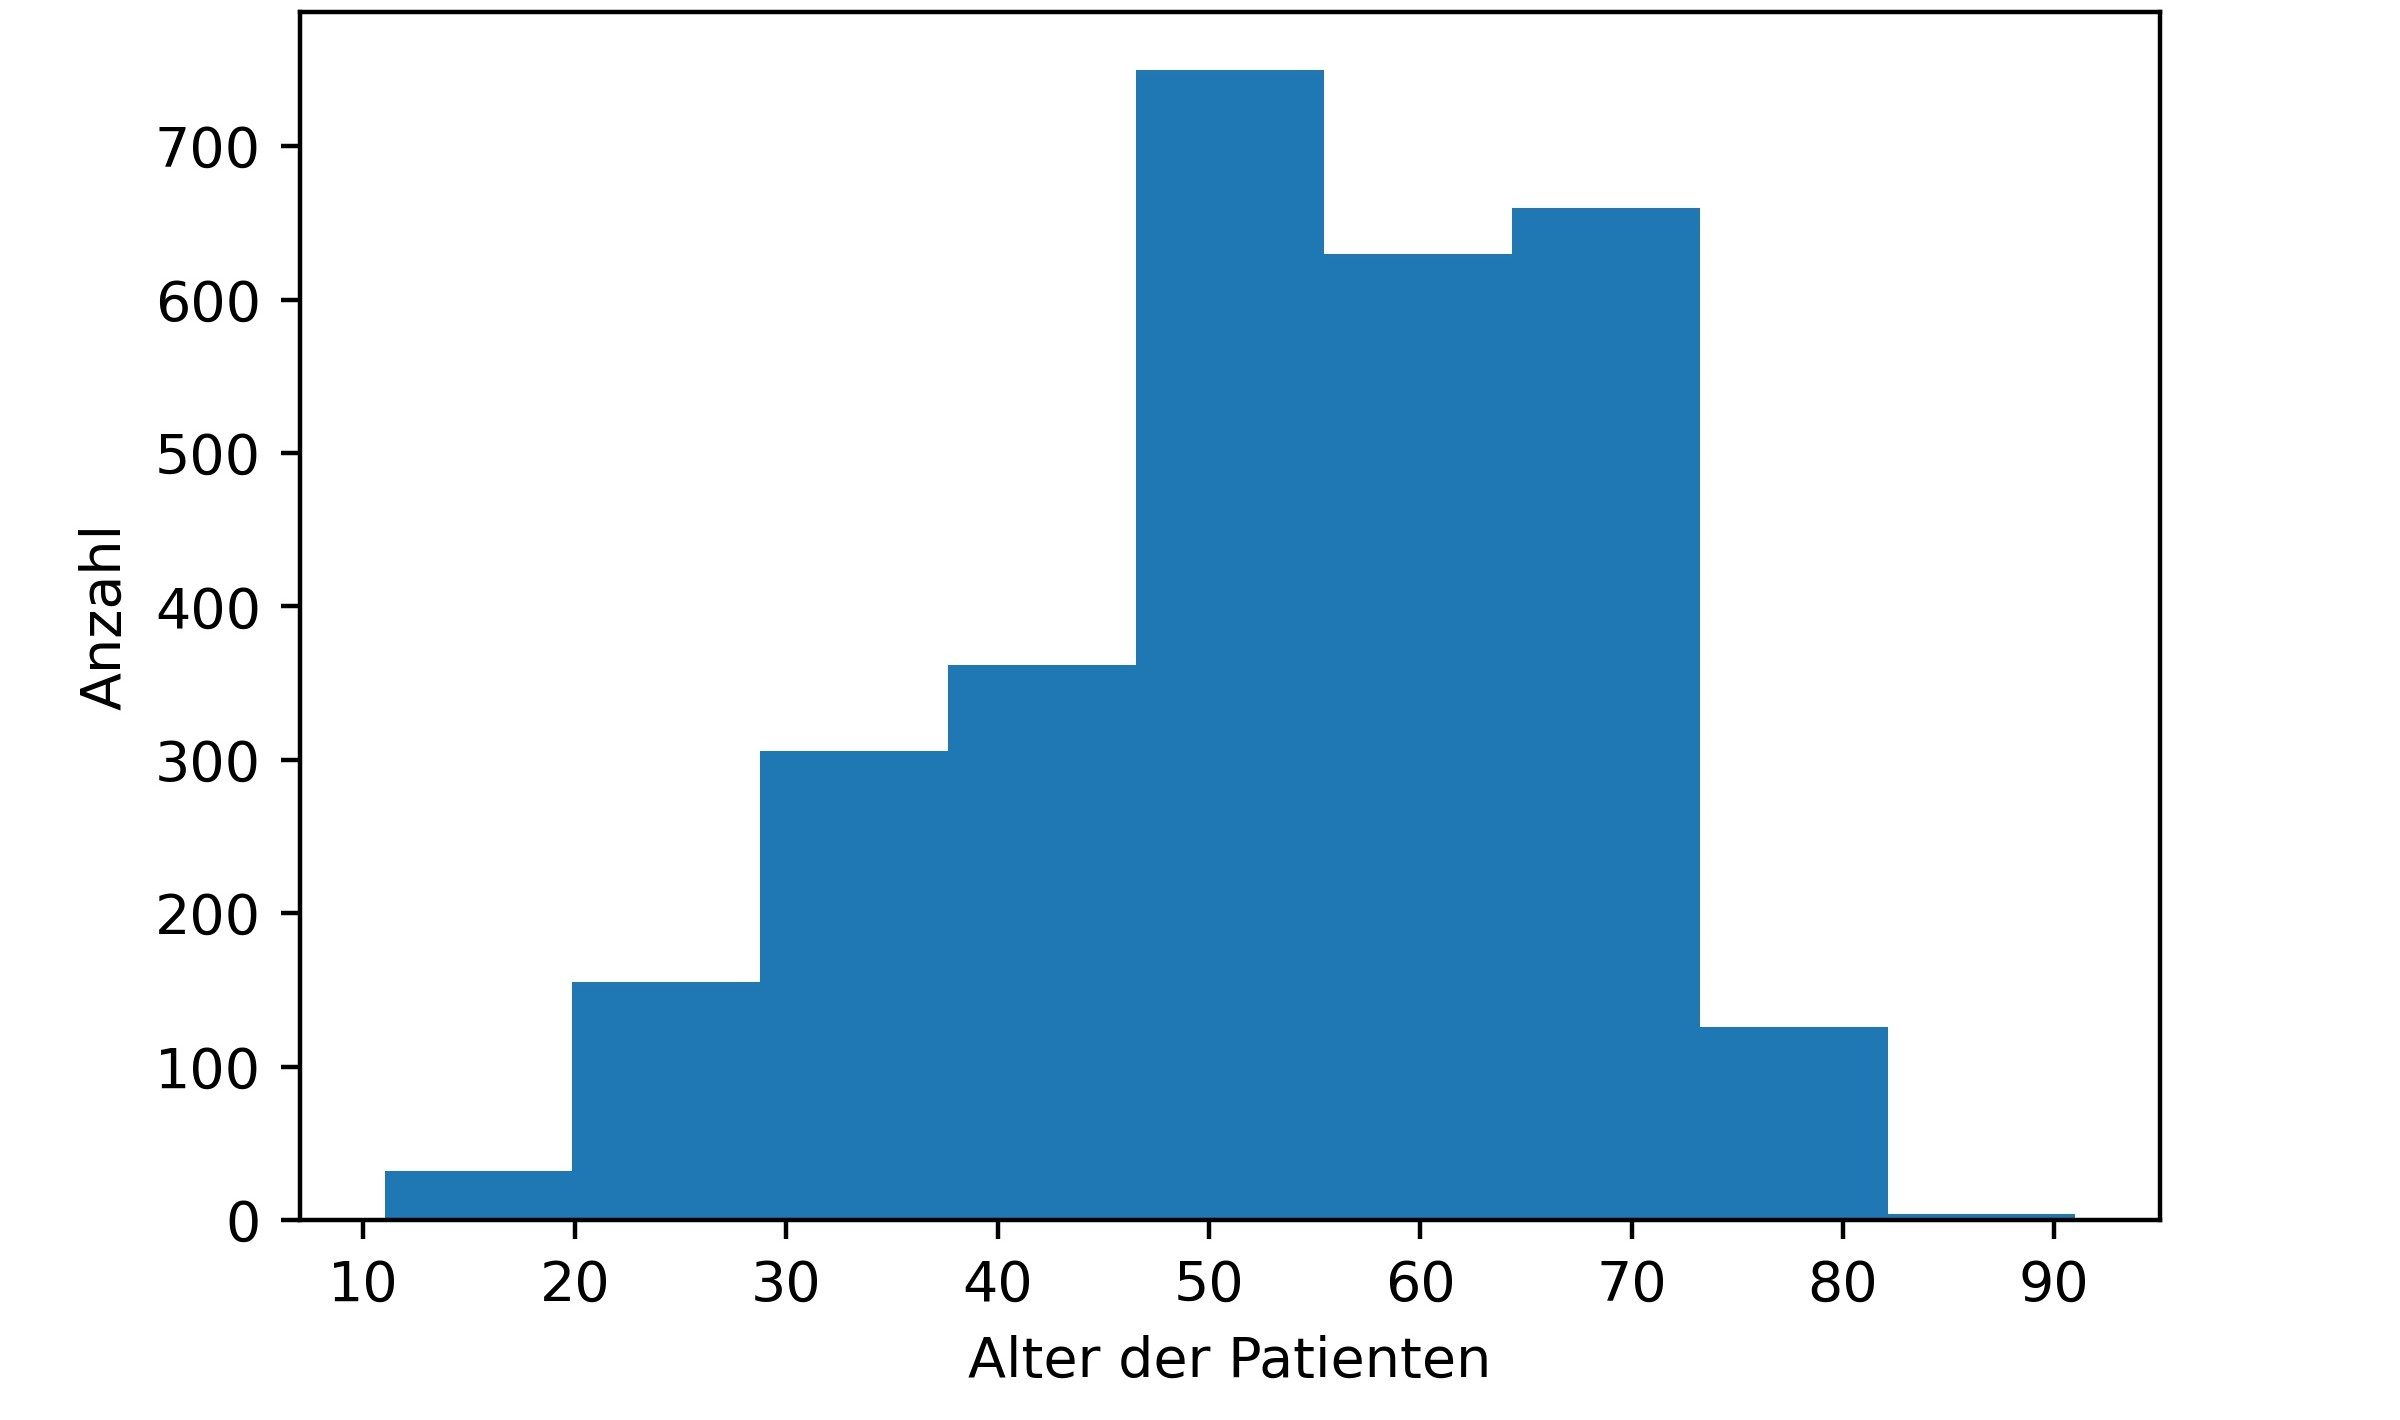
\includegraphics[width=0.80\textwidth]{./Bilder/MetadataAltershistogramm.jpg}
	\end{center}
	\caption{Histogramm der Demographie des Datensatzes.}%
	\label{fig:Altershist}%
\end{figure}

Die manuelle Annotation ist in 0.5 Sekunden Segmente unterteilt. Die Analyse der manuellen Annotationen ergibt eine durchschnittliche Anzahl von LM im Schlaf von 266. Am häufigsten aufgetreten sind Aufzeichnungen mit 17 annotierten LM. Der durchschnittliche PLMS/h-Wert liegt bei $9.95 * 10^{-3}$. Dabei haben 875 Dateien einen Wert von Null.

\section{Wahl des Detektors}\label{chap:WahldesDetektors}
Um die gefundenen Metriken anzuwenden, soll für diese Arbeit ein Detektor umgesetzt werden. 
Augenscheinlich sind die vorgeschlagenen Detektoren in der Tabelle im Stand der Technik ausreichend performant, sodass hier auf die Entwicklung eines neuen Detektors verzichtet werden kann.
Die am weitesten verbreitete Methode – und somit auch am weitesten entwickelte Methode – nutzt eine EMG-Signalvorverarbeitung und einen doppelten Schwellwertvergleich mit Nachbearbeitung des Annotationssignals. Der Vorteil eines Schwellwertvergleiches liegt außerdem in einer geringen Rechenlaufzeit, da keine Modelle trainiert werden müssen und die Berechnungen leicht zu parallelisieren sind. 
Der Algorithmus von Huang et al. wurde nur auf einem sehr kleinen Datensatz getestet und benötigt eine hohe EMG-Qualität, da ein absoluter Schwellwert implementiert ist. Die Variante von Moore baut auf den Erkenntnissen von Ferri et al., Tauchmann und Wetter et al. auf. 

Also wurde für den Rahmen dieser Arbeit der Detektor von Moore et al. implementiert. Es gibt zwar eine weiterentwickelte Variante von Alvarez-Estevez, welche bessere Ergebnisse liefert, diese ist jedoch wesentlich komplizierter aufgebaut und schwieriger vergleichbar mit den anderen Detektoren, da die Metriken anhand von einsekündigen Segmenten erstellt wurden. 
Da es in dieser Arbeit hauptsächlich um die Untersuchung der Metriken geht, ist die von Moore et al. erreicht Klassifikationsgüte ausreichend. 

Die Funktionsstruktur des Programms wurde im Stand der Technik beschrieben und ist hier in Python implementiert. Deswegen werden hier nur die Anpassungen beschrieben:
Beim Einlesen der Dateien werden die leeren Annotationssignale übersprungen, da diese keinen Informationsgehalt bieten. Die beiden EMG-Signale der Beine werden laut \cite{Moore} zu einem Signal zusammengeführt. Die Signale für beide Beine einzeln zu berechnen wie in \cite{alvarez} funktioniert hier nicht, da für die Nachbearbeitung der Annotationssignale ein Grundrauschen des kombinierten Signals gebraucht wird.
Das RMS-Signal und der gleitende Mittelwert werden mit einer Randeffektanpassung errechnet, um das Signal nicht an den Rändern zu verfälschen. 
Hierbei werden die erkannten LM gelöscht, welche vor dem „Licht aus“-Zeitpunkt und nach „Licht An“-Zeitpunkt stattgefunden haben, da diese auch nicht in dem manuellen Annotationssignal vorhanden sind. 
Es werden auch Beinbewegungen entfernt, welche laut AASM die Maximallänge von 10 Sekunden überschreiten. Durch das Zusammenführen der beiden Beine dürfen laut AASM alternierende Bewegungen zusammengefasst werden. Mit zusätzlicher Filterung sind Beinbewegungen im Signal von mehr als 15 Sekunden möglich. Für bessere Vergleichbarkeit mit der Literatur wurde der Wert aus der Arbeit von Moore et al. implementiert. 

Bei der Umsetzung des Detektors wurde die adaptive Filterung der Elektrokardiogrammstörung und die Löschung der Beinbewegungen in der Nähe von atembezogenen Events verzichtet, da die benötigten Signale nicht zur Verfügung gestellt wurden. 

Die automatischen und manuellen Annotationen werden mit den jeweiligen Start- und Endzeitpunkten in einer CSV-Datei gespeichert.
Ein separates Programm kann die Annotationssignale aus den CSV-Dateien auslesen und daraus die Metriken bestimmen. Hier wird auch das Signal zu den Schlafstadien geladen, um die LM zu entfernen, die nicht im Schlaf stattgefunden haben. 
Des Weiteren gibt es ein Programm, welches alle pro Nacht berechneten Metriken einliest und zwischen den Nächten vergleicht.

\section{Funktion des Detektors}
An folgendem Beispiel lässt sich gut die Funktionsweise des Detektors anhand des Schwellwertes und die folgende Nachbearbeitung nachvollziehen. In Abbildung \ref{fig:detectorWorking2} ist oben das vorbearbeitete EMG-Signals (blau) und der davon abhängige dynamische obere Schwellwert zu erkennen. In dem Annotationssignal darunter ist ein Zwischenergebnis des Detektors zu sehen, bei dem alle Zeiträume annotiert wurden, bei denen das EMG-Signal über dem Schwellwert liegt. 
Das unterste Bild zeigt das finale automatische (orange) Annotationssignal nach der Nachbearbeitung. Dazu ist die manuelle Annotation zum Vergleich in blau auf der gleichen Achse dargestellt. 



\begin{figure}[!ht]%
	\begin{center}
	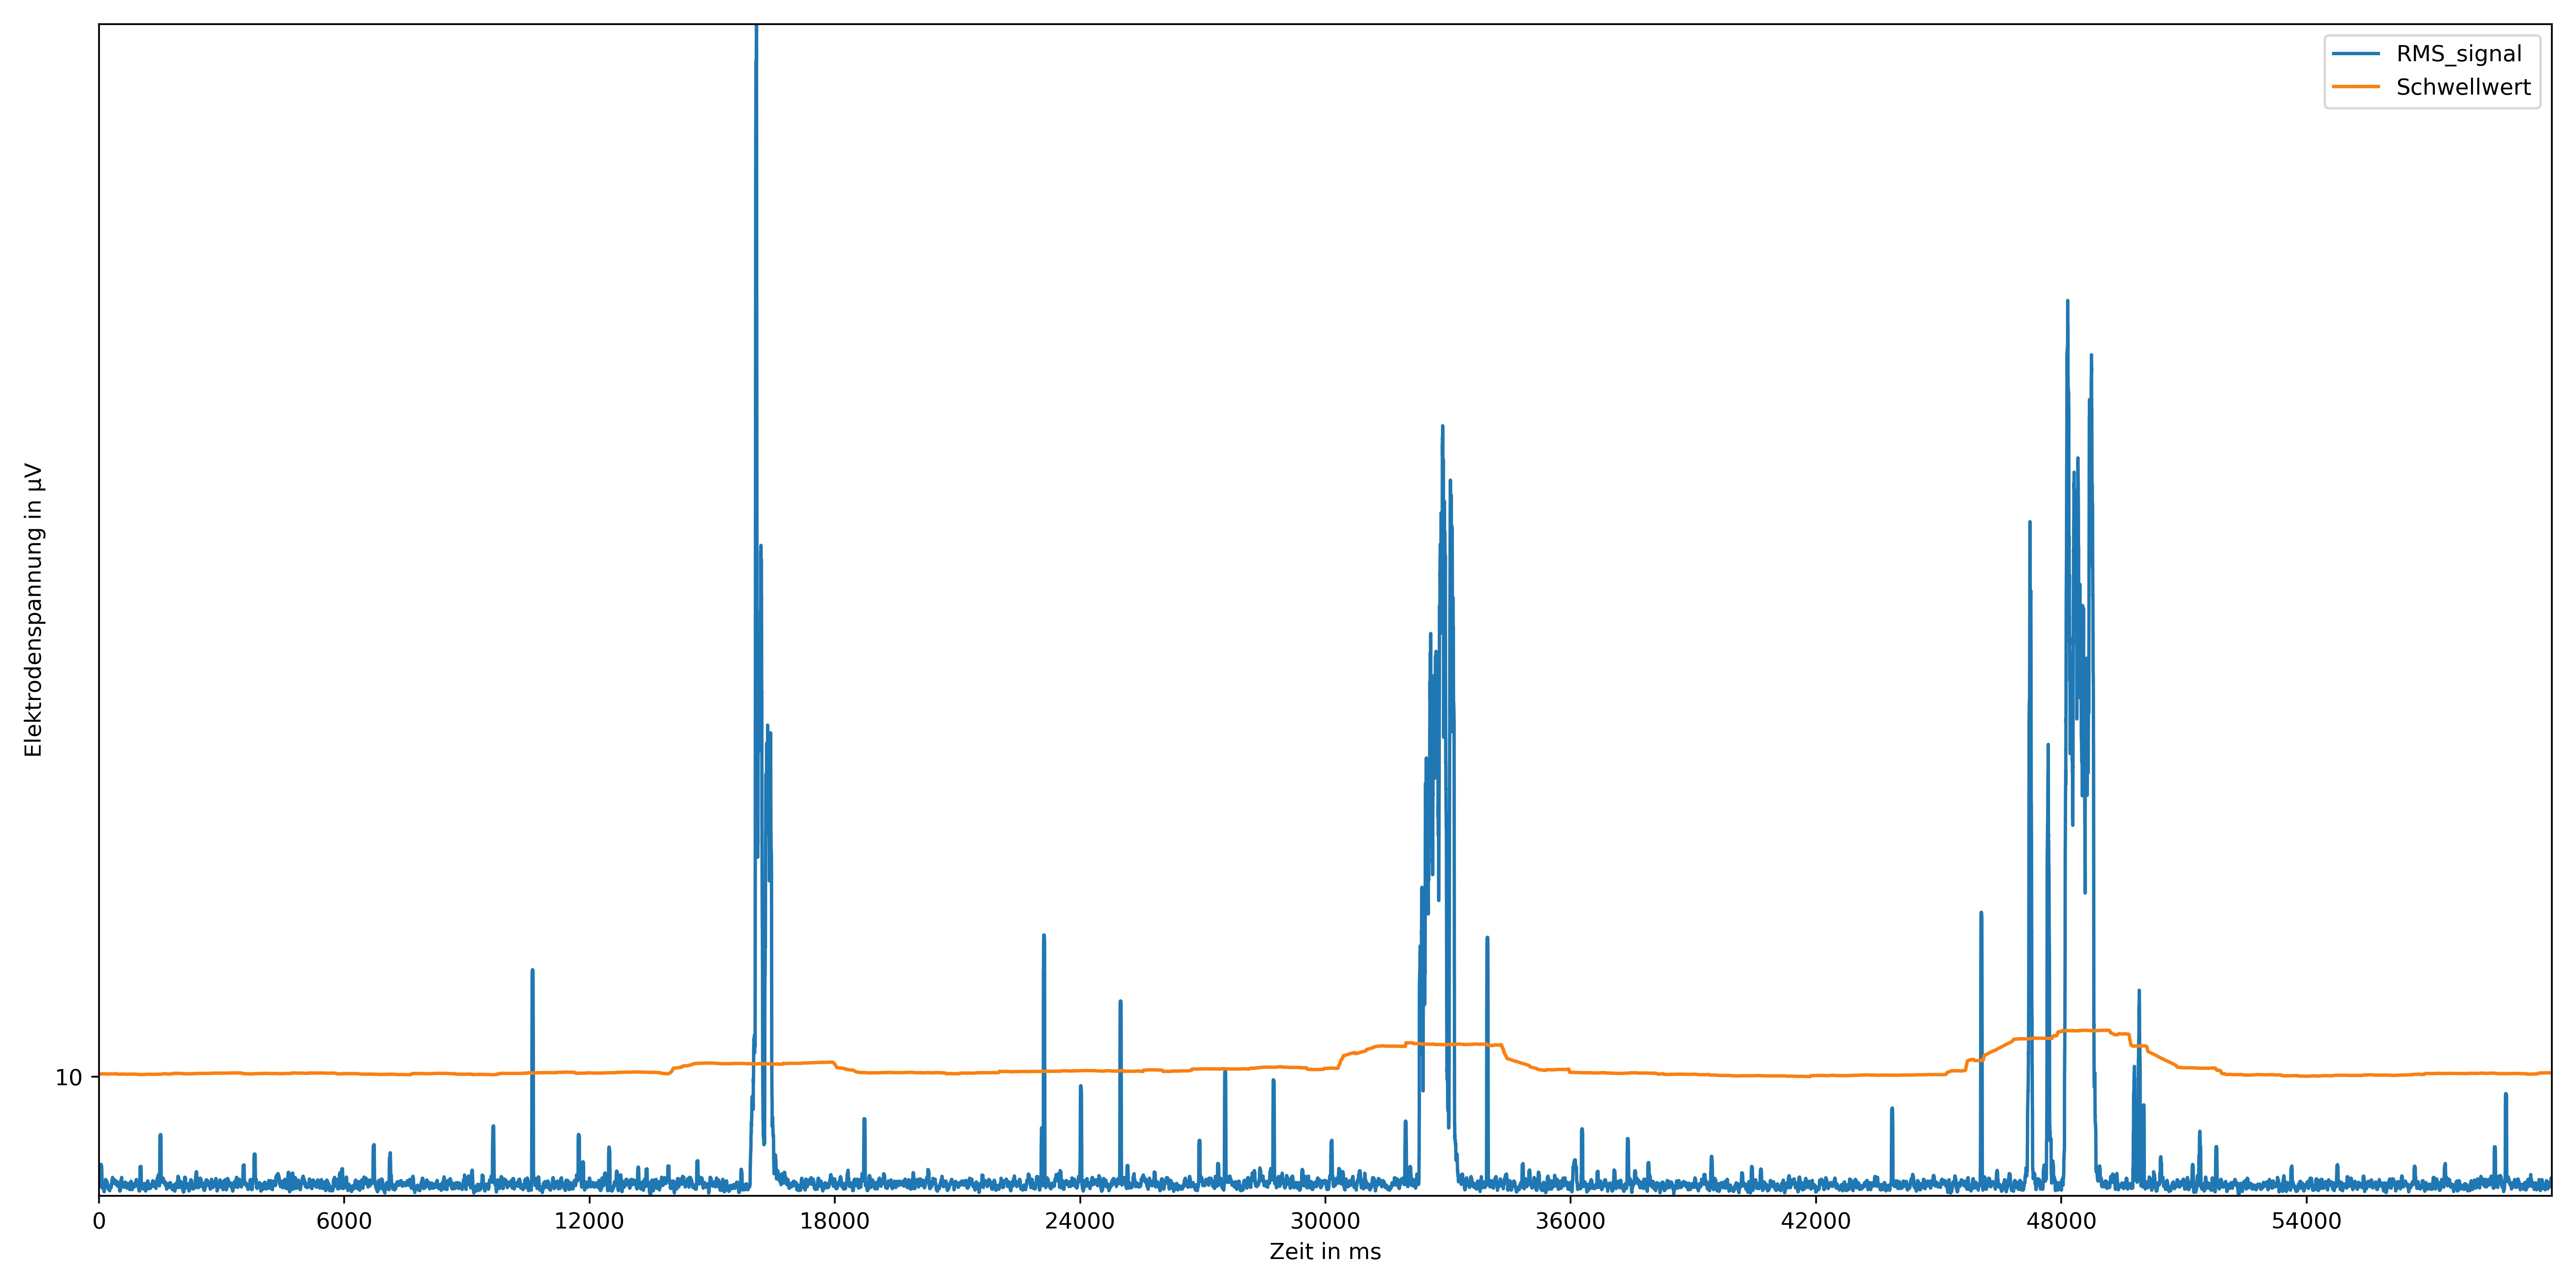
\includegraphics[width=0.80\textwidth]{./Bilder/detectorWorkEMGacq_002944221.edf2870000,60000.jpg}
	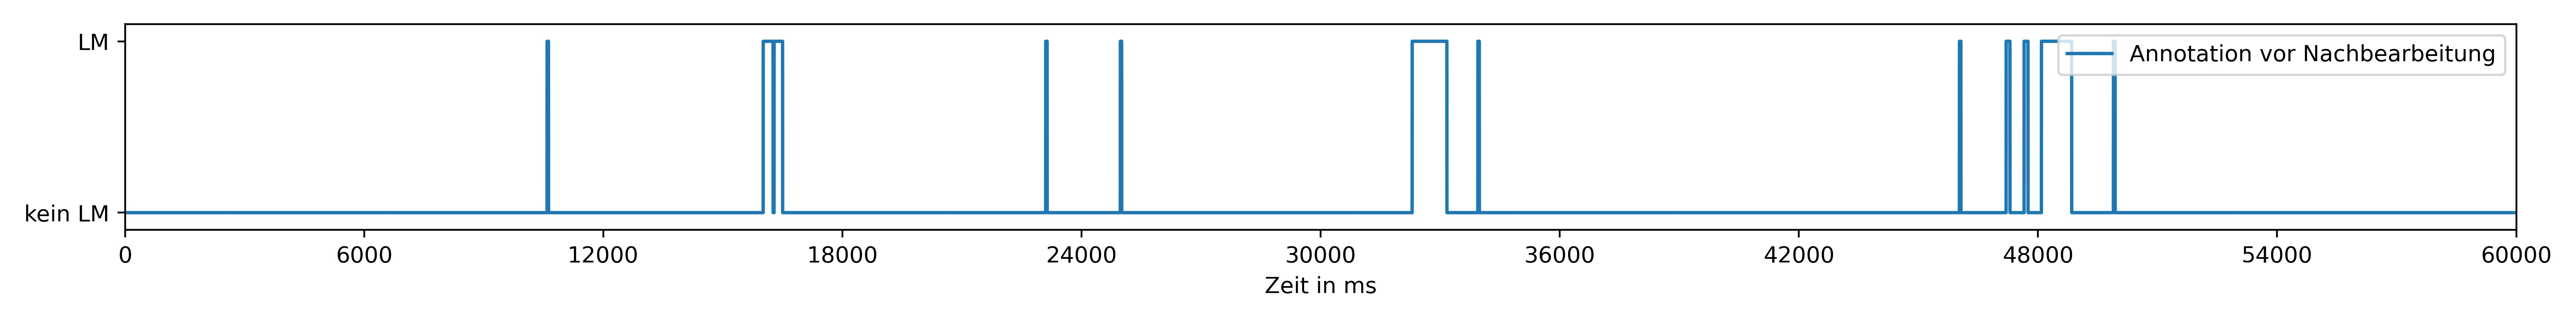
\includegraphics[width=0.80\textwidth]{./Bilder/detectorWork2acq_002944221.edf2870000,60000.jpg}
	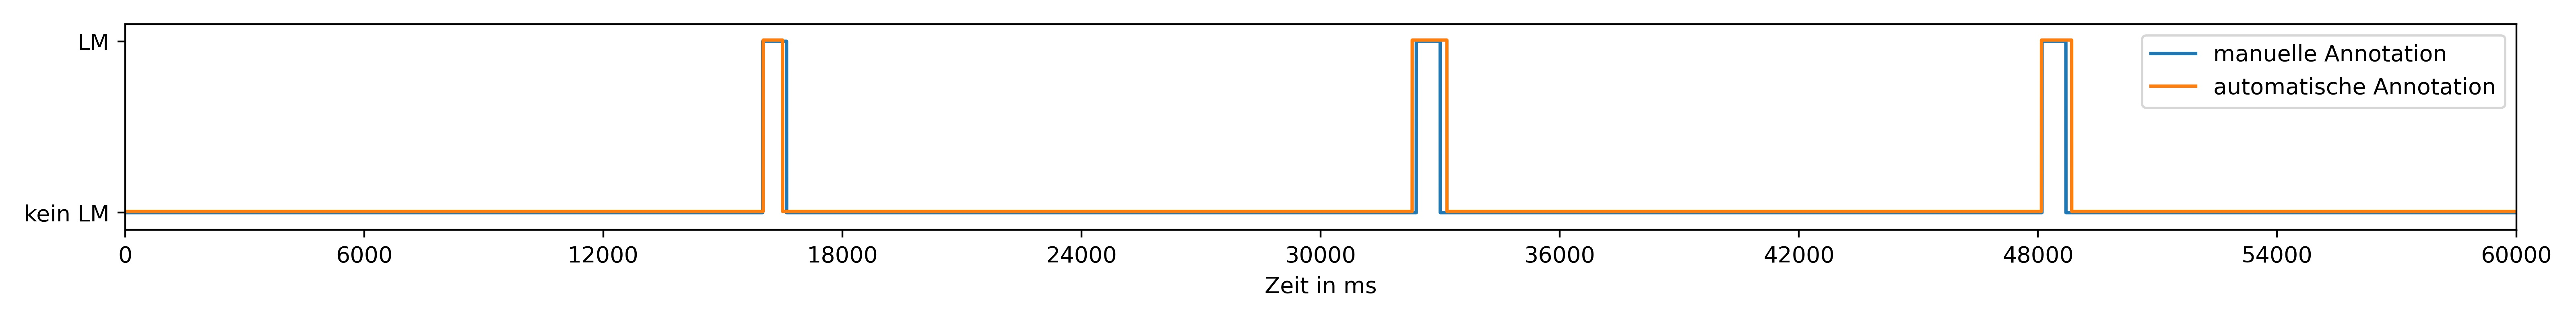
\includegraphics[width=0.80\textwidth]{./Bilder/detectorWorkacq_002944221.edf2870000,60000.jpg}
	\end{center}
	\caption{Veranschaulichung der Funktionsweise des implementierten Detektors: vorverarbeitetes EMG-Signal mit oberem Schwellwert (oben), Zwischenergebnis des Annotationssignals vor der Nachbearbeitung (mittig), finale automatische und manuelle Annotation zum Vergleich (unten). Die Abtastfrequenz beträgt 200 Hz.}%
	\label{fig:detectorWorking2}%
\end{figure}

Damit bei unregelmäßigem EMG-Signal keine \glspl{LM} erkannt werden, passt sich der dynamische Schwellwert an die veränderte Qualität an. 
In Abbildung \ref{fig:detectorWorking} lässt sich der Vorteil eines dynamischen Schwellwertes veranschaulichen. Für den dargestellten Zeitraum wurden manuell keine Beinbewegungen annotiert.

\begin{figure}[!ht]%
	\begin{center}
	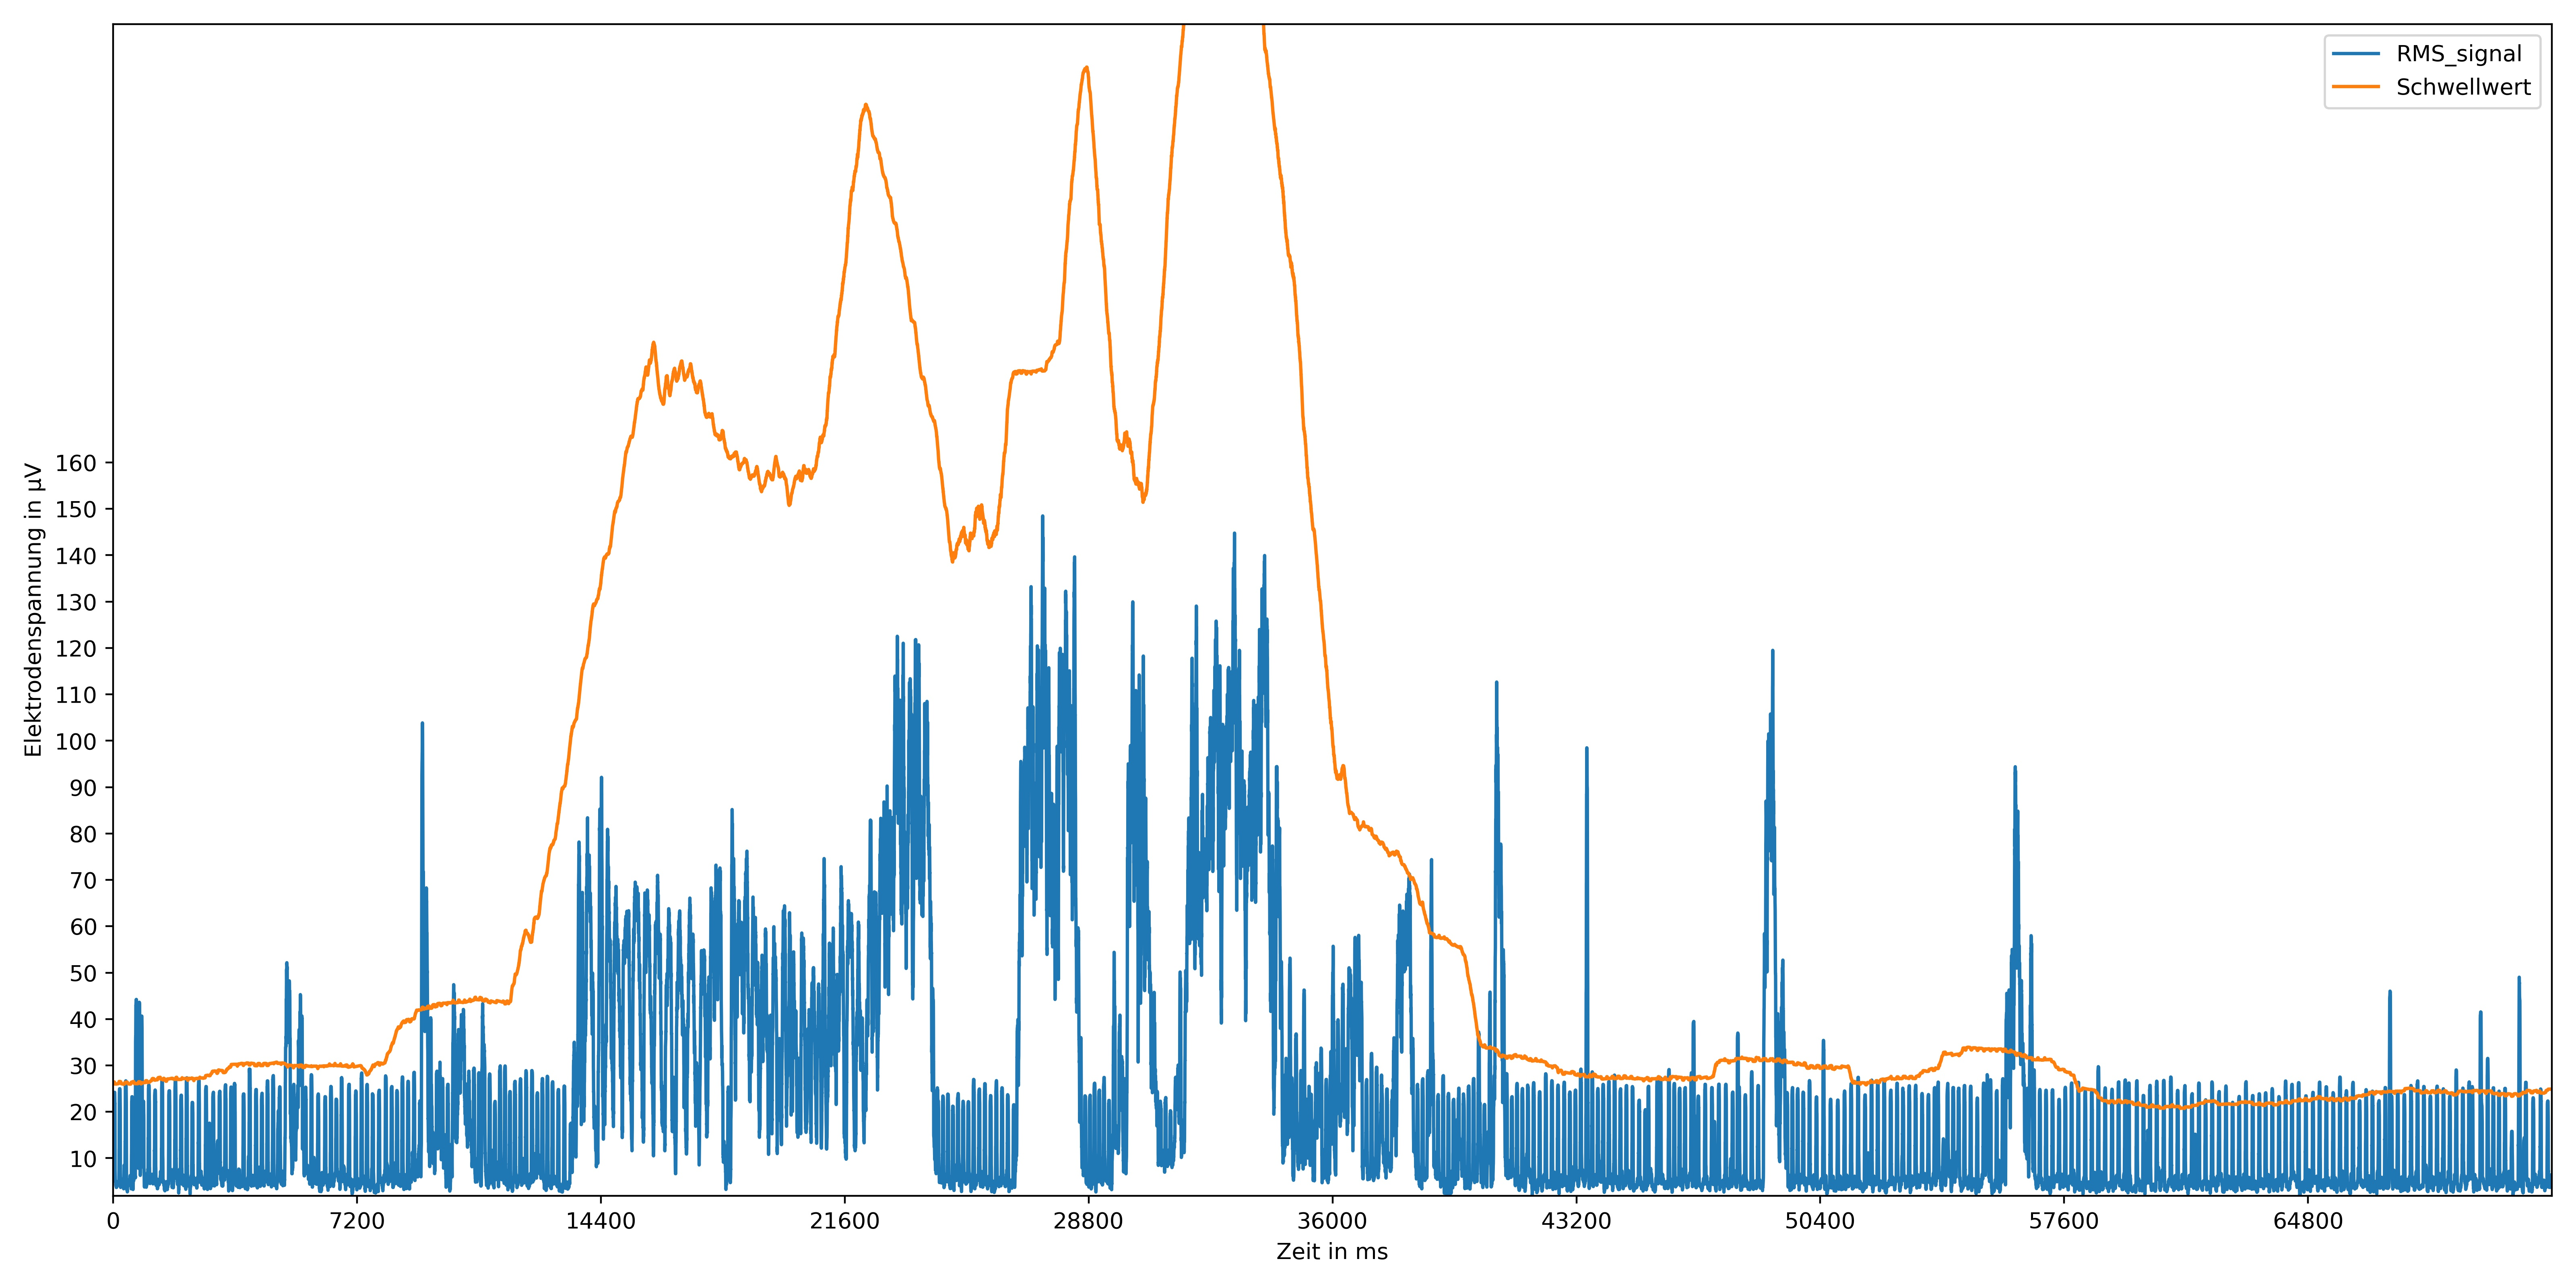
\includegraphics[width=0.80\textwidth]{./Bilder/vorrübergehendesRauschenEMGacq_002963603.edf108000,72000.jpg}
	
	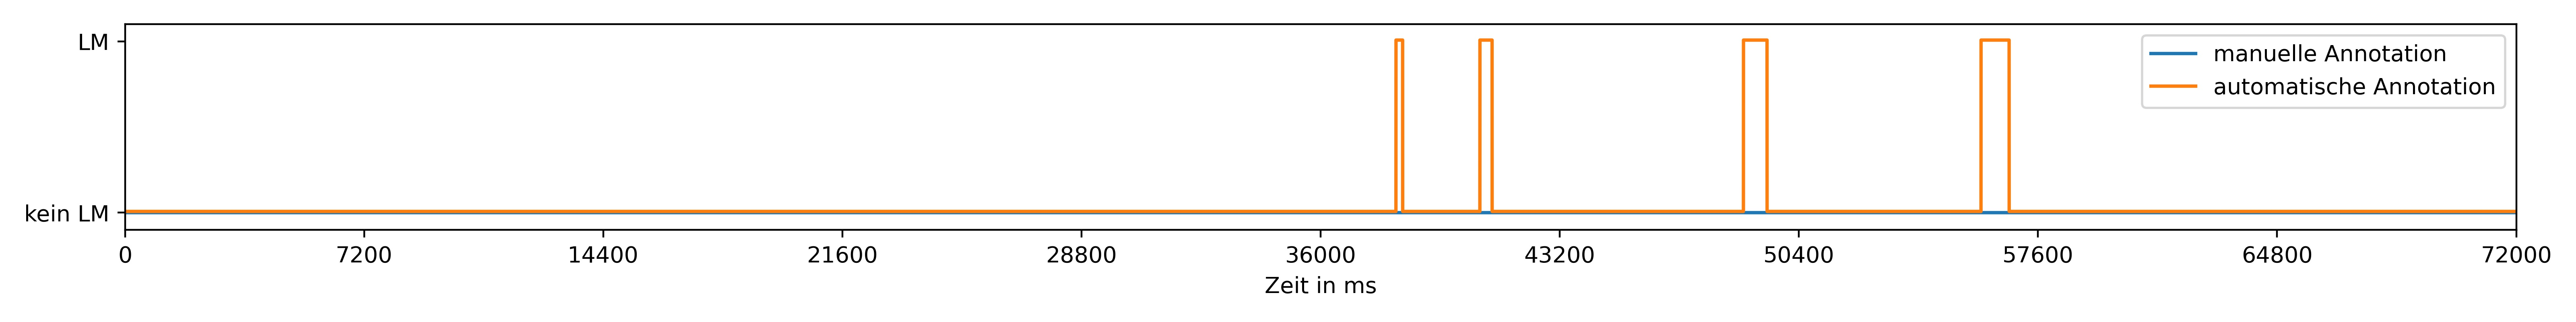
\includegraphics[width=0.80\textwidth]{./Bilder/vorrübergehendesRauschenacq_002963603.edf108000,72000.jpg}
	\end{center}
	\caption{Ausschnitt eines unregelmäßigen EMG-Signals zur Veranschaulichung der dynamischen Anpassung des Schwellwertes (oben) und die daraus resultierende automatischer Annotation (unten). Die Abtastfrequenz beträgt 200 Hz.}%
	\label{fig:detectorWorking}%
\end{figure}


Das folgende Signal (Abb. \ref{fig:EKG}) zeigt einen Ausschnitt einer EKG Störung mit einer Herzfrequenz von ungefähr einem Hertz und den daraus resultierenden erhöhten oberen Schwellwert. Durch diese Einkopplungen sind Beinbewegungen nicht mehr klar erkennbar.

\begin{figure}[!ht]%
	\begin{center}
	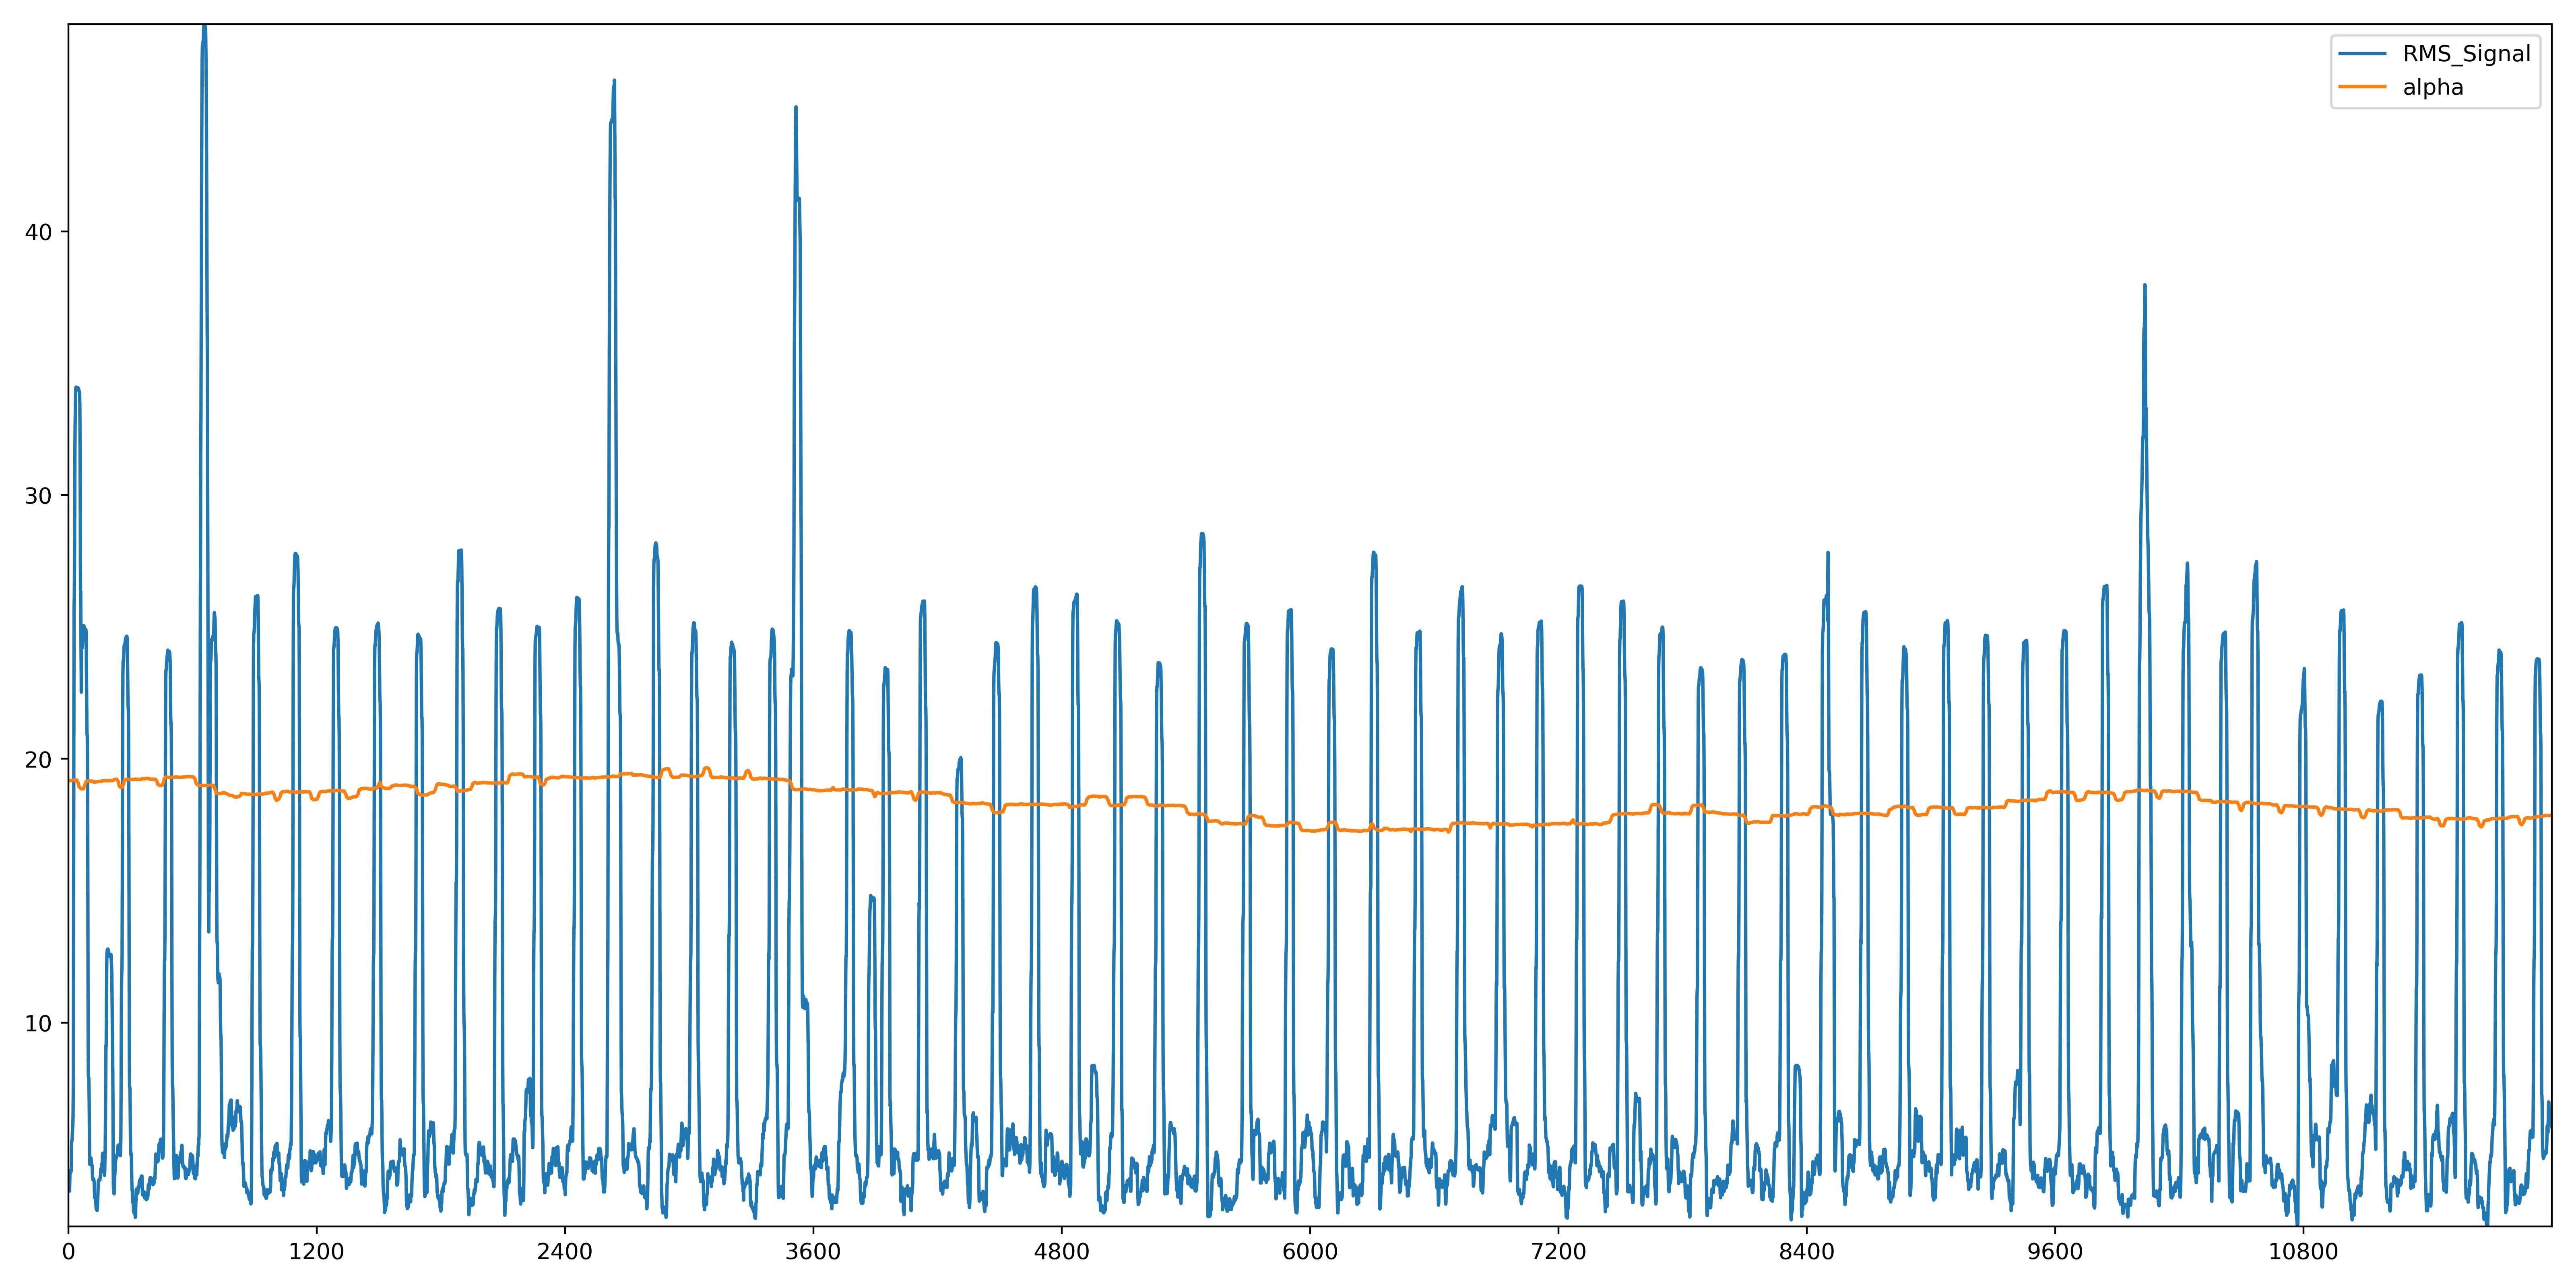
\includegraphics[width=0.80\textwidth]{./Bilder/maybeNoiseNoIdeaWhatHappenedEMGacq_002963603.edf276000,12000.jpg}
	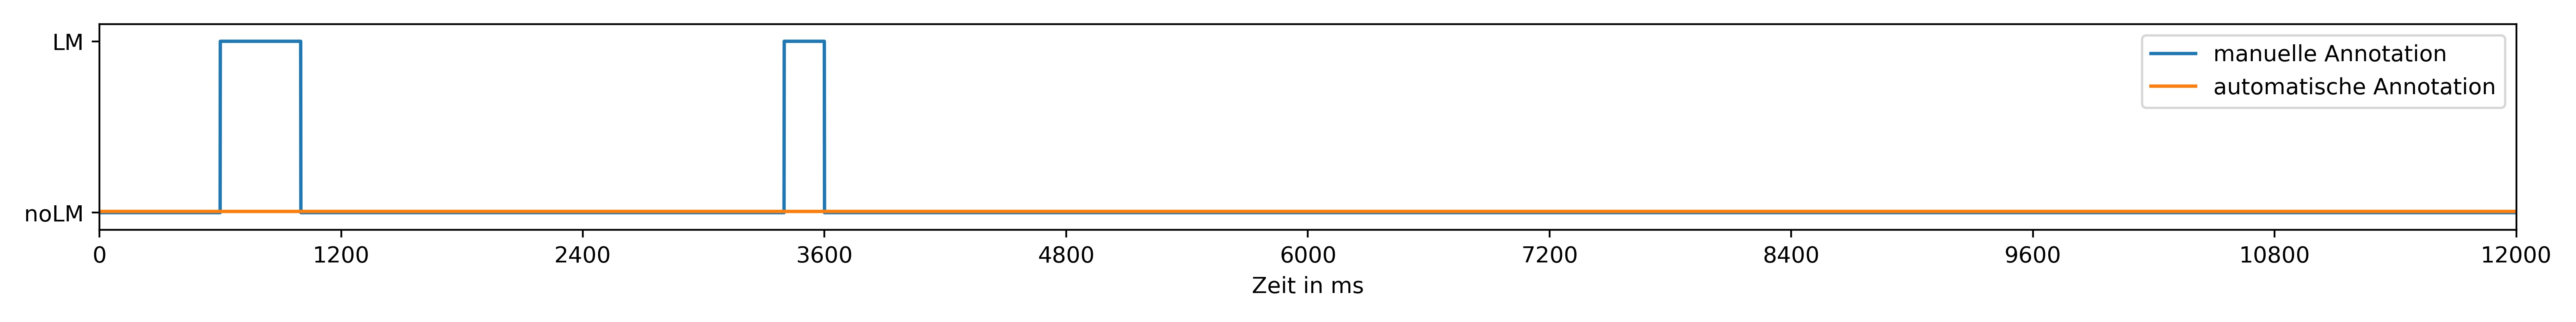
\includegraphics[width=0.80\textwidth]{./Bilder/maybeNoiseNoIdeaWhatHappenedacq_002963603.edf276000,12000.jpg}
	\end{center}
	\caption{EMG-Signal mit EKG Einkopplung (oben), bei der die manuell annotierten Beinbewegungen von dem Detektor nicht erkannt wurden.}%
	\label{fig:EKG}%
\end{figure}

